% Chapter 1

\chapter{Introducción General} % Main chapter title
En este capítulo se describe la motivación del trabajo y sus objetivos, con una pequeña explicación de algunos conceptos fundamentales para entenderlo.

\label{Chapter1} % For referencing the chapter elsewhere, use \ref{Chapter1} 
%\label{IntroGeneral}

%----------------------------------------------------------------------------------------

% Define some commands to keep the formatting separated from the content 
\newcommand{\keyword}[1]{\textbf{#1}}
\newcommand{\tabhead}[1]{\textbf{#1}}
\newcommand{\code}[1]{\texttt{#1}}
\newcommand{\file}[1]{\texttt{\bfseries#1}}
\newcommand{\option}[1]{\texttt{\itshape#1}}
\newcommand{\grados}{$^{\circ}$}

%----------------------------------------------------------------------------------------

%\section{Introducción}

%----------------------------------------------------------------------------------------
\section{Descripción general del trabajo y conceptos clave}

El trabajo desarrollado consiste en un sistema adquisidor de datos con los sensores necesarios para una medición de potencia eléctrica, en otras palabras, un medidor digital de energía eléctrica. El trabajo fue desarrollado para SERVAIND S.A. que es una empresa privada localizada en Argentina.

El término medida es utilizado para describir el acto de determinar el valor o tamaño de una cantidad por ejemplo una corriente. Hay un gran número de tipos de cantidades en el campo de la ingeniería que necesitan ser medidas o expresadas en el trabajo día a día. Esto incluye cantidades físicas, mecánicas y eléctricas por ejemplo. De modo de almacenar y comparar estas magnitudes de cantidad algunas magnitudes deben ser tomadas como base o unidad \citep{book:1689974}. Estas unidades medidas son de interés y por lo tanto se almacenan en el medidor digital.

La adquisición de datos o adquisición de señales consiste en la toma de muestras del mundo real (sistema analógico) para generar datos que puedan ser manipulados por un ordenador u otros dispositivos electrónicos (sistema digital). Se requiere una etapa de acondicionamiento, que adecua la señal a niveles compatibles con el elemento que hace la transformación a señal digital.\cite{NIDataAdquisition}

Un convertidor de señal analógica a digital (ADC) es un dispositivo electrónico capaz de convertir una señal analógica, ya sea de tensión o corriente, en una señal digital mediante un cuantificador y codificador.


\subsection{Sistemas electrónicos para mediciones eléctricas}

Las aplicaciones más tempranas de computadores digitales a problemas de sistemas de potencia datan de alrededor de 1940. La mayoría de las aplicaciones tempranas estaban limitadas en alcance debido a la pequeña capacidad de las tarjetas calculadoras usadas en ese período. Computadoras digitales de larga escala estuvieron disponibles a mediados de 1950, y el éxito inicial de programas de flujo de carga llevó al desarrollo de programas para cálculos de corto circuitos y estabilidad \citep{761852}.

Los medidores electrónicos digitalizan las variables medidas vía un ADC sigma delta  de alta resolución. La técnica de diseño de estos medidores digitales está influenciada por tres grandes factores: el costo , eficiencia y tamaño. Mientras que el costo se ve influenciado por la capacidad de compra del cliente, la eficiencia y el tamaño se encuentran sujetos a estándares como los establecidos por la IEC (International Electrotechnical Commission) \cite{articleDM}.

\begin{figure}[h]
	\centering
	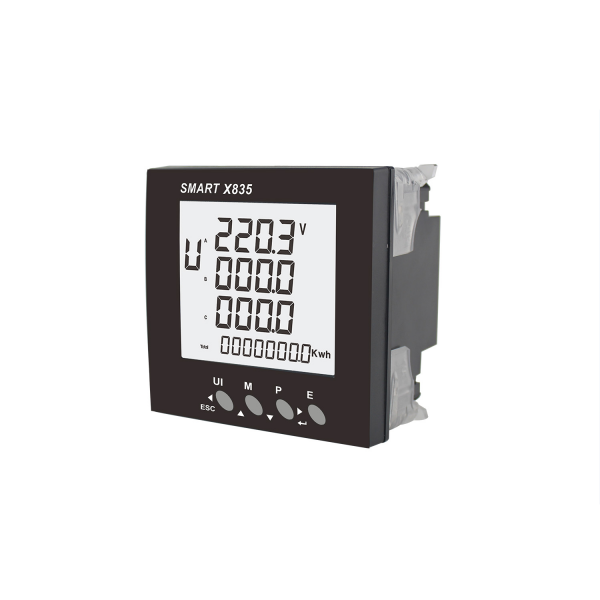
\includegraphics[width=55mm,keepaspectratio]{Figures/3931_1.png}
	\caption{Medidor electrónico comercial.}
	\label{fig:texmaker}
\end{figure}

La exactitud del medidor eléctrico digital depende de la precisión del circuito analógico de entrada analógica, la del conversor analógico-digital y la de los cálculos digitales \citep{Hribik2004DigitalPA}.

Los convertidores analógicos-digitales basados en la modulación sigma - delta son económicamente viables para convertidores de alta resolución (mayores que 12 bits), por lo que son  usados en el circuito integrado de procesadores de señales.

La modulación sigma-delta fue introducida en 1962 y no ganaría importancia hasta recientes desarrollos en tecnologías VLSI (integración a escala muy grande) que proveen fines prácticos para implementar complejos circuitos de procesamiento de señales \citep{book:28601}.

\section{Motivación}

En la actualidad se pueden encontrar en el mercado internacional múltiples módulos electrónicos de bajo costo con puertos de comunicación para la medición de energía eléctrica como así también medidores digitales de energía de diferentes marcas para diferentes entornos, lo que nos permite pensar que un dispositivo similar podría ser fabricado en la Argentina.

Los módulos de medición pueden servir como un monitoreo de primera instancia y funcionar como un método preventivo de fallas, dado que los parámetros de consumo dan una idea de estado de las máquinas.  El módulo de la figura \ref{fig:pzem04} fue usado en un trabajo de grado para un local comercial cuyo resultados pueden verse en la figura \ref{fig:graficoW}.  

\begin{figure}[h]
	\centering
	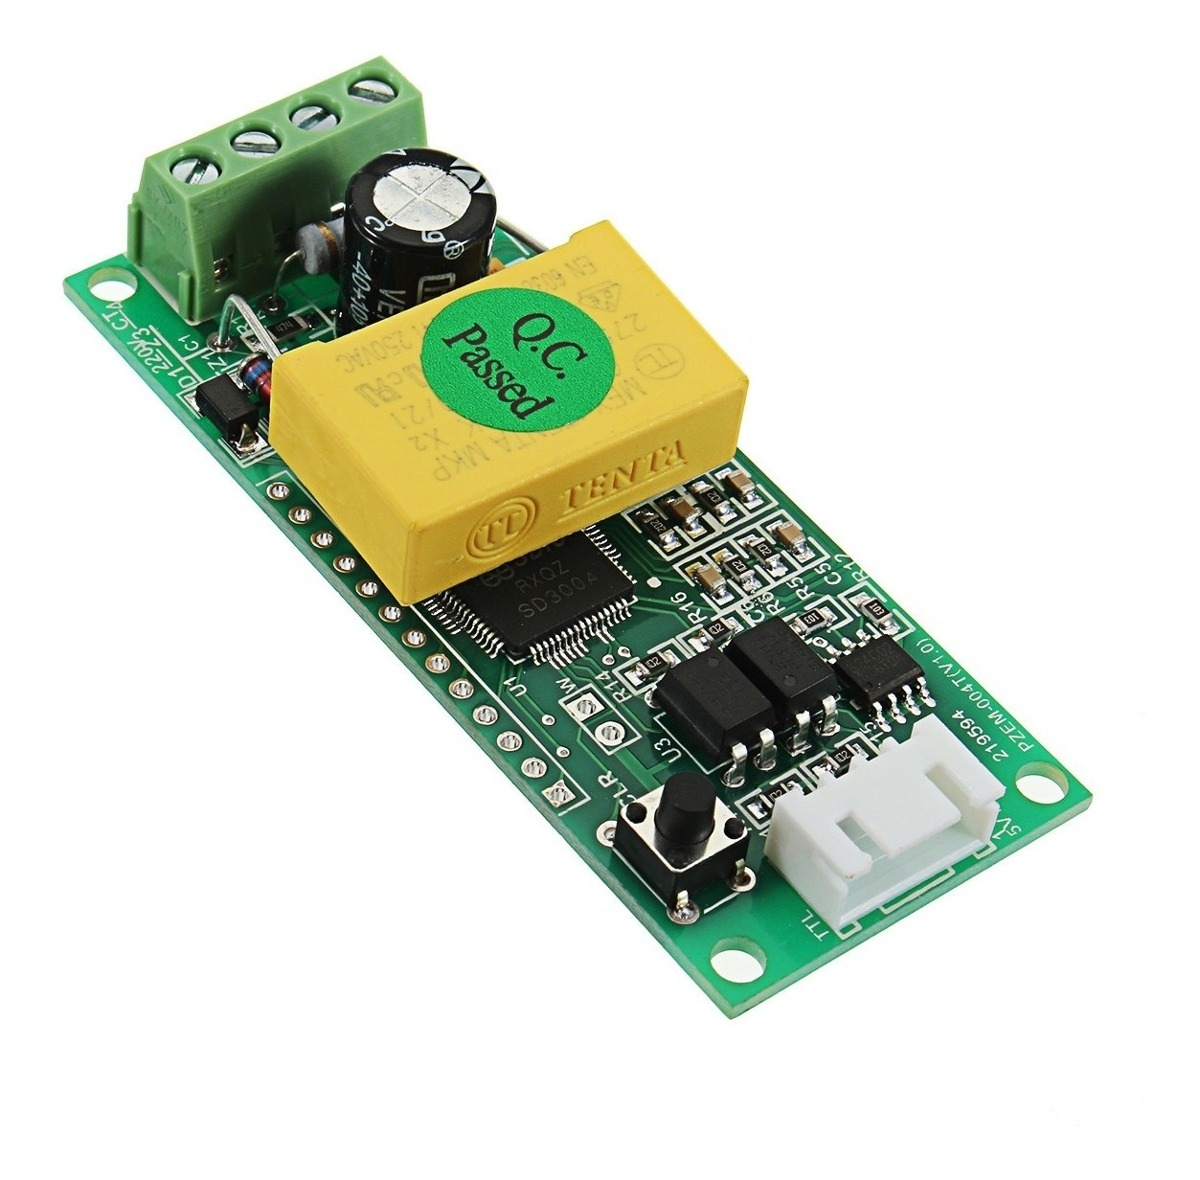
\includegraphics[width=80mm,keepaspectratio]{Figures/pzeem004.jpg}
	\caption{Módulo de medición de energía eléctrica con comunicación serie universal.}
	\label{fig:pzem04}
\end{figure}

Estos módulos se consiguen únicamente en el mercado internacional de modo que hay que importarlos, lo que presenta una barrera para una herramienta de monitoreo simple.

\begin{figure}[!h]
	\centering
	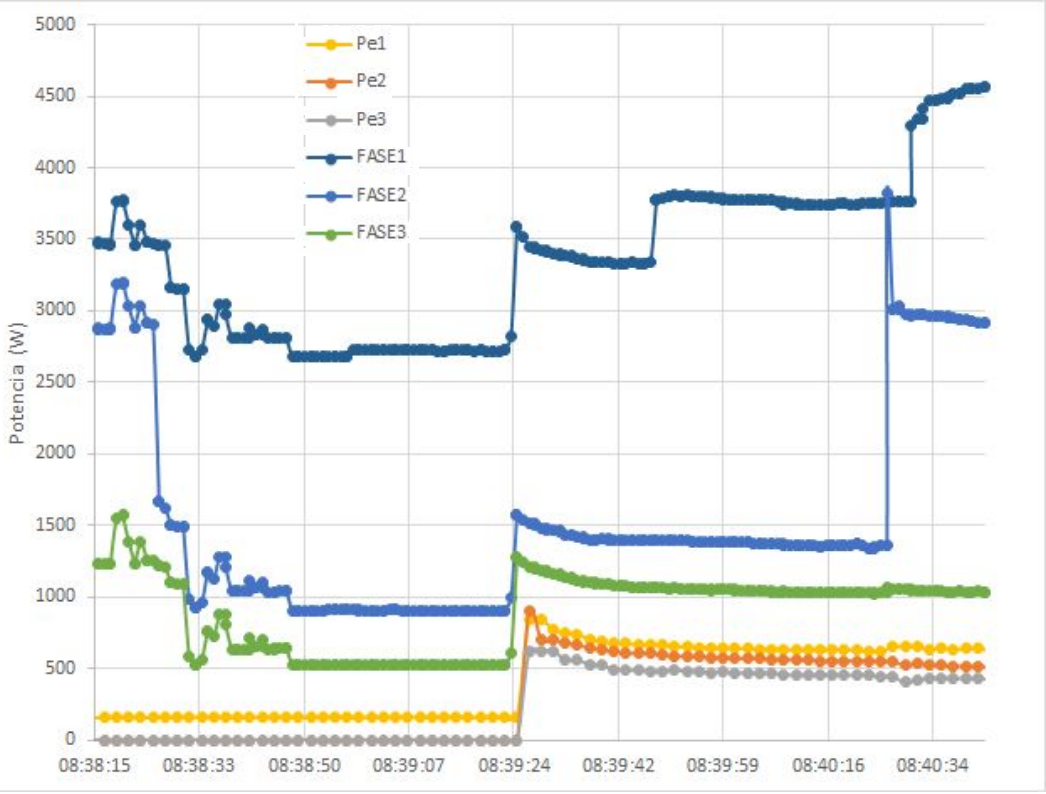
\includegraphics[width=120mm,keepaspectratio]{Figures/potencia_ej.png}
	\caption{Gráfico de medición de potencia que muestran el encendido de un frigorífico.}
	\label{fig:graficoW}
\end{figure}

Estas gráficas sirvieron para realizar observaciones como el encendido de un motor trifásico y malfuncionamiento de equipos de refrigeración.
 

Desde el punto de vista de la empresa privada, el trabajo se planteó ante la necesidad de cuantificar consumos energéticos de procesos industriales para supervisar la alimentación de equipos de control o de medición. También como una alternativa a un producto anterior que solo medía consumos de corriente continua. En suma la necesidad de hacer uso de la herramienta y poseer los medios necesarios para fabricar la electrónica de manera local  impulsaron el trabajo realizado.

\section{Objetivos y alcance}


\subsection{Objetivos del desarrollo}

El objetivo del trabajo fue el desarrollo de un dispositivo de medición basado en un microcontrolador de la familia MSP430 en conjunto con un ADC SOC (\textit{system on chip}). Se pretende lograr un dispositivo comercial similar a aquellos elaborados anteriormente por la empresa privada, por lo que las dimensiones del PCB (\textit{printed circuit board}) deberán ajustarse a los utilizados por las carcasas estándar que utiliza la empresa, como puede verse en la figura \ref{fig:disp_emp}.

\begin{figure}[h]
	\centering
	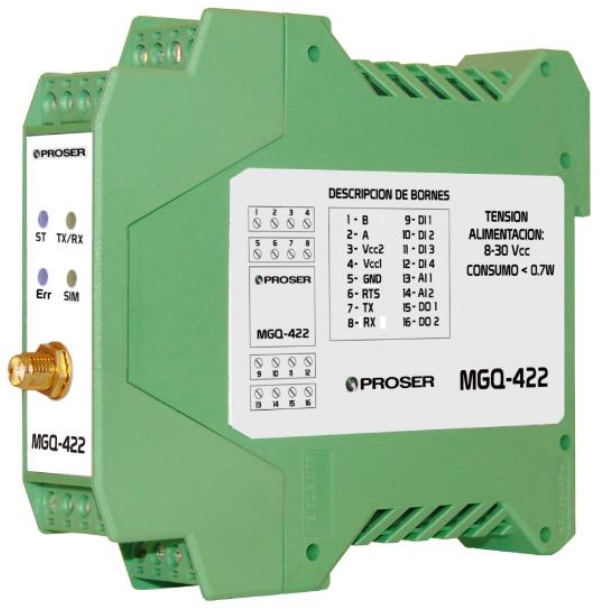
\includegraphics[width=80mm,keepaspectratio]{Figures/dispositivo_empresa.png}
	\caption{Ejemplo de dispositivo fabricado por la SERVAIND S.A.}
	\label{fig:disp_emp}
\end{figure}

Además, se esperaba que el firmware manejara protocolo modbus y comunicara las variables medidas a través de los puertos de comunicación. Físicamente se pretendío que el dispositivo fuera capaz de comunicar por puertos serie RS-232 y RS-485, y que este pudiera funcionar en un ambiente industrial (el dispositivo tendría que ser robusto).


\subsection{Alcances}


%----------------------------------------------------------------------------------------

El trabajo abarco el planteo, diseño y fabricación de un pcb. Asimismo, incluye la selección de componentes, la elaboración del esquemático de conexiones lógicas y la elaboración del pcb y su diseño para la fabricación. Ademas se debió elaborar un prototipo y realizar testeos sobre este.

También se esperaba realizar un firmware para el funcionamiento del dispositivo, teniendo en cuenta que el software debía incluir métodos de configuración para un futuro usuario.





